\documentclass{LaBRI_poster}

\usepackage[utf8]{inputenc}
\usepackage{subfig}
\usepackage[export]{adjustbox}
\usepackage{amsmath,enumerate}
\usepackage{multicol}
%---------------------------------------------------------
% Choose the following to decide whether or not you need to include the INRIA Logo.

\INRIAtrue
%\INRIAfalse

\title{SIFT descriptor to set landmarks on biological images}
%\subtitle{La fable ``Le Faucon et le Chapon''}

\author{Van Linh LE$^{1}$, Marie BEURTON-AIMAR$^{1}$, Adrien KRAHENBUHL$^{2}$, Nicolas PARISEY$^{3}$}
% Vous êtes probablement seul auteur de votre poster.
% Pour les coauteurs des résultats, il vaut mieux les citer avec les résultats.

\institute{$^{1}$LaBRI - UMR 5800, Univ. Bordeaux; $^{2}$ICube - UMR 7357, Univ. Strasbourg; $^{3}$INRA - IGEPP UMR 1349}
% indiquer son équipe.

\def\Put(#1,#2)#3{\leavevmode\makebox(0,0){\put(#1,#2){#3}}}

\begin{document}

\begin{frame}[t] % The whole poster is enclosed in one beamer frame

% The whole poster consists of sections of one, two or three columns. Choose the appropriate width :
% \onecolwidth, \twocolwidth, \threecolwidth, or \fourcolwidth
% correspond to the width of one column when there are 1, 2, 3 or 4 columns in parallel.
% You can even use \twothirdcolwidth when you want to distribute 
% two columns with 2/3 and 1/3
%
% spacing empty columns of size \sepwidth should be inserted on both sides and between columns if you want to have a clean positioning of the columns.

\begin{columns}[t] 

\begin{column}{\sepwidth}\end{column} % Empty spacer column

\begin{column}{\onecolwidth}
 \begin{alertblock}{Context}
	Morphometry analysis is a way to distinguish the characteristics of organisms, i.e \textit{shape, size, form,...}. It is used to appreciate the covariances between the ecological factors and the organisms. Landmark-based morphometry is known as one of the approaches to analyze the characteristics of organisms. Finding enough landmarks can give to biologists a comprehensive description of the organism. This work focuses on the automatic identification of landmarks on 2D biological images.
 \end{alertblock}
 
 \begin{block}{Landmarks}
 	\begin{itemize}
  		\item Morphometric landmarks are points of interest in the biological object. They usually stay along the outline of the image.\\[0.3cm]
  		\item Landmarks characterize specificities through the shape most often linked to biological information,\\[0.3cm]
  		\item They are usually \textbf{defined} \textbf{manually} by biologists,\\[0.3cm]
  		\item Images at the right side show manual landmarks in \textbf{beetle mandibles} belonging to our sample:\\
  		\hspace{0.5cm}$16$ and $18$ manual landmarks have been defined for each left mandible and right mandible, respectively.
  	\end{itemize}
 	\Put(1450,0){\hspace{1cm}{\LARGE{\textcolor{labriTopRed}{\textbf{How to locate the landmarks automatically}?}}}}
  	\Put(1000,7){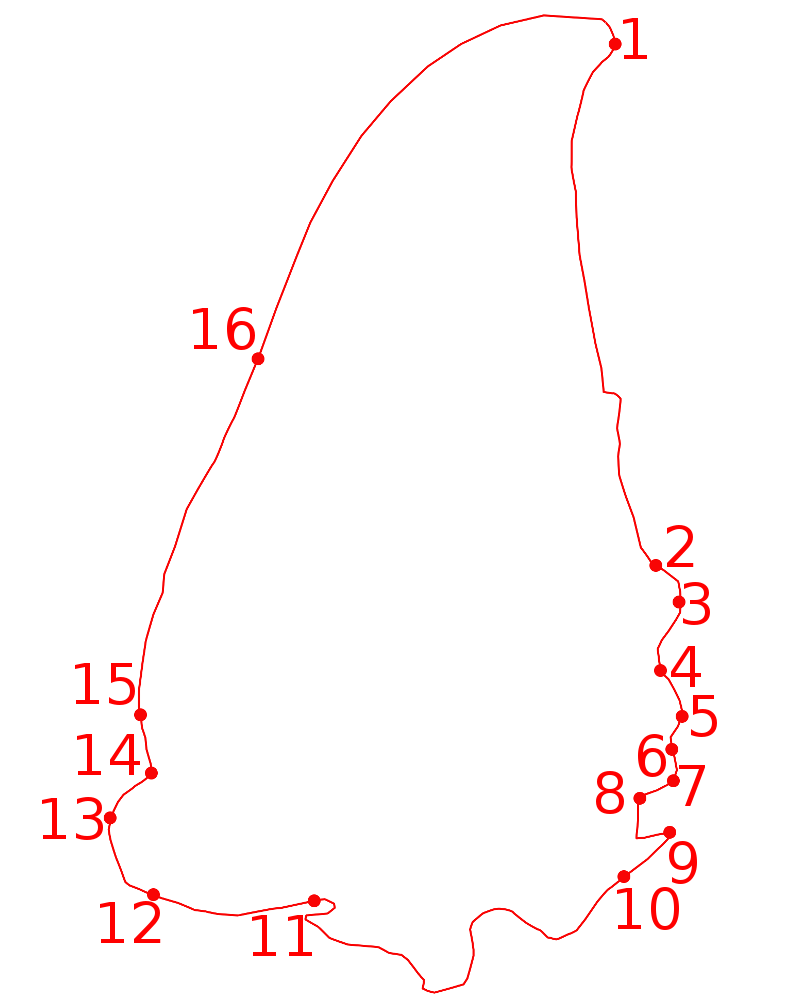
\includegraphics[scale=.38]{images/mlandmarksline}}
    \Put(1200,7){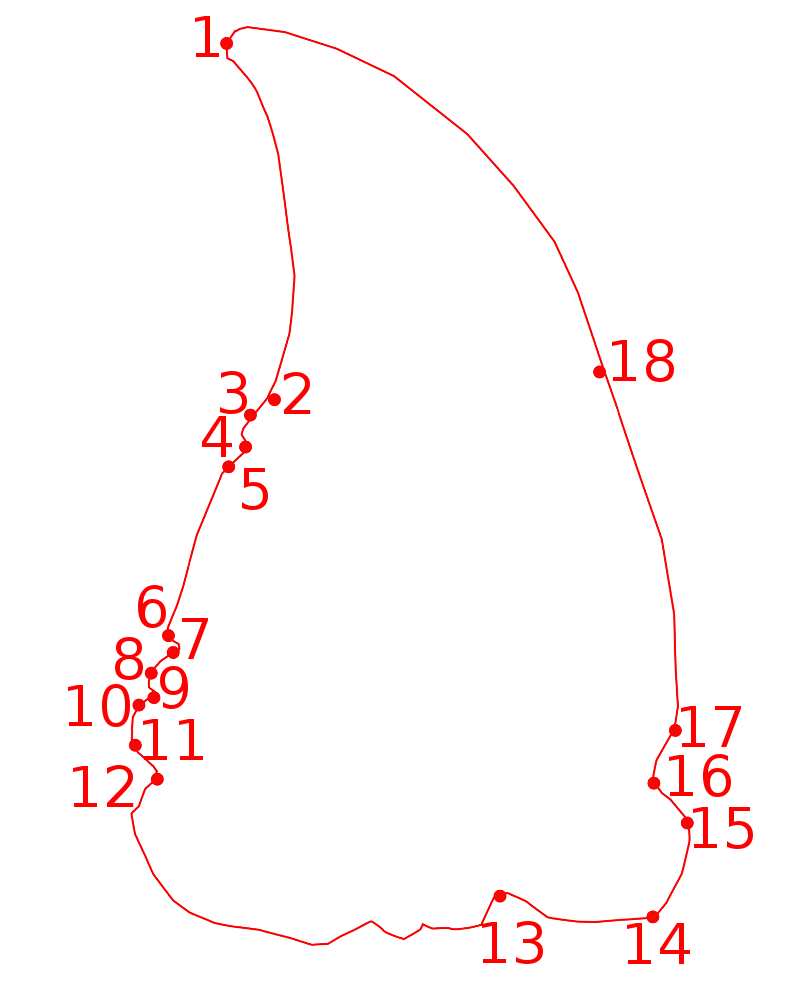
\includegraphics[scale=.38]{images/mglandmarksline}}
    ~\\[2.0cm]
    
    ~\\[2cm]
 \end{block}
\end{column}

\begin{column}{\sepwidth}\end{column} % Empty spacer column

\end{columns}

% ------------ Horizontal separation for changing number of columns in the width ------------

\begin{columns}[t] 

\begin{column}{\sepwidth}\end{column} % Empty spacer column
\begin{column}{\threecolwidth}
\begin{block}{Mandibles and manual landmarks}
\begin{figure}[h]
\centering
\subfloat[Left mandible]{\label{figrbox2}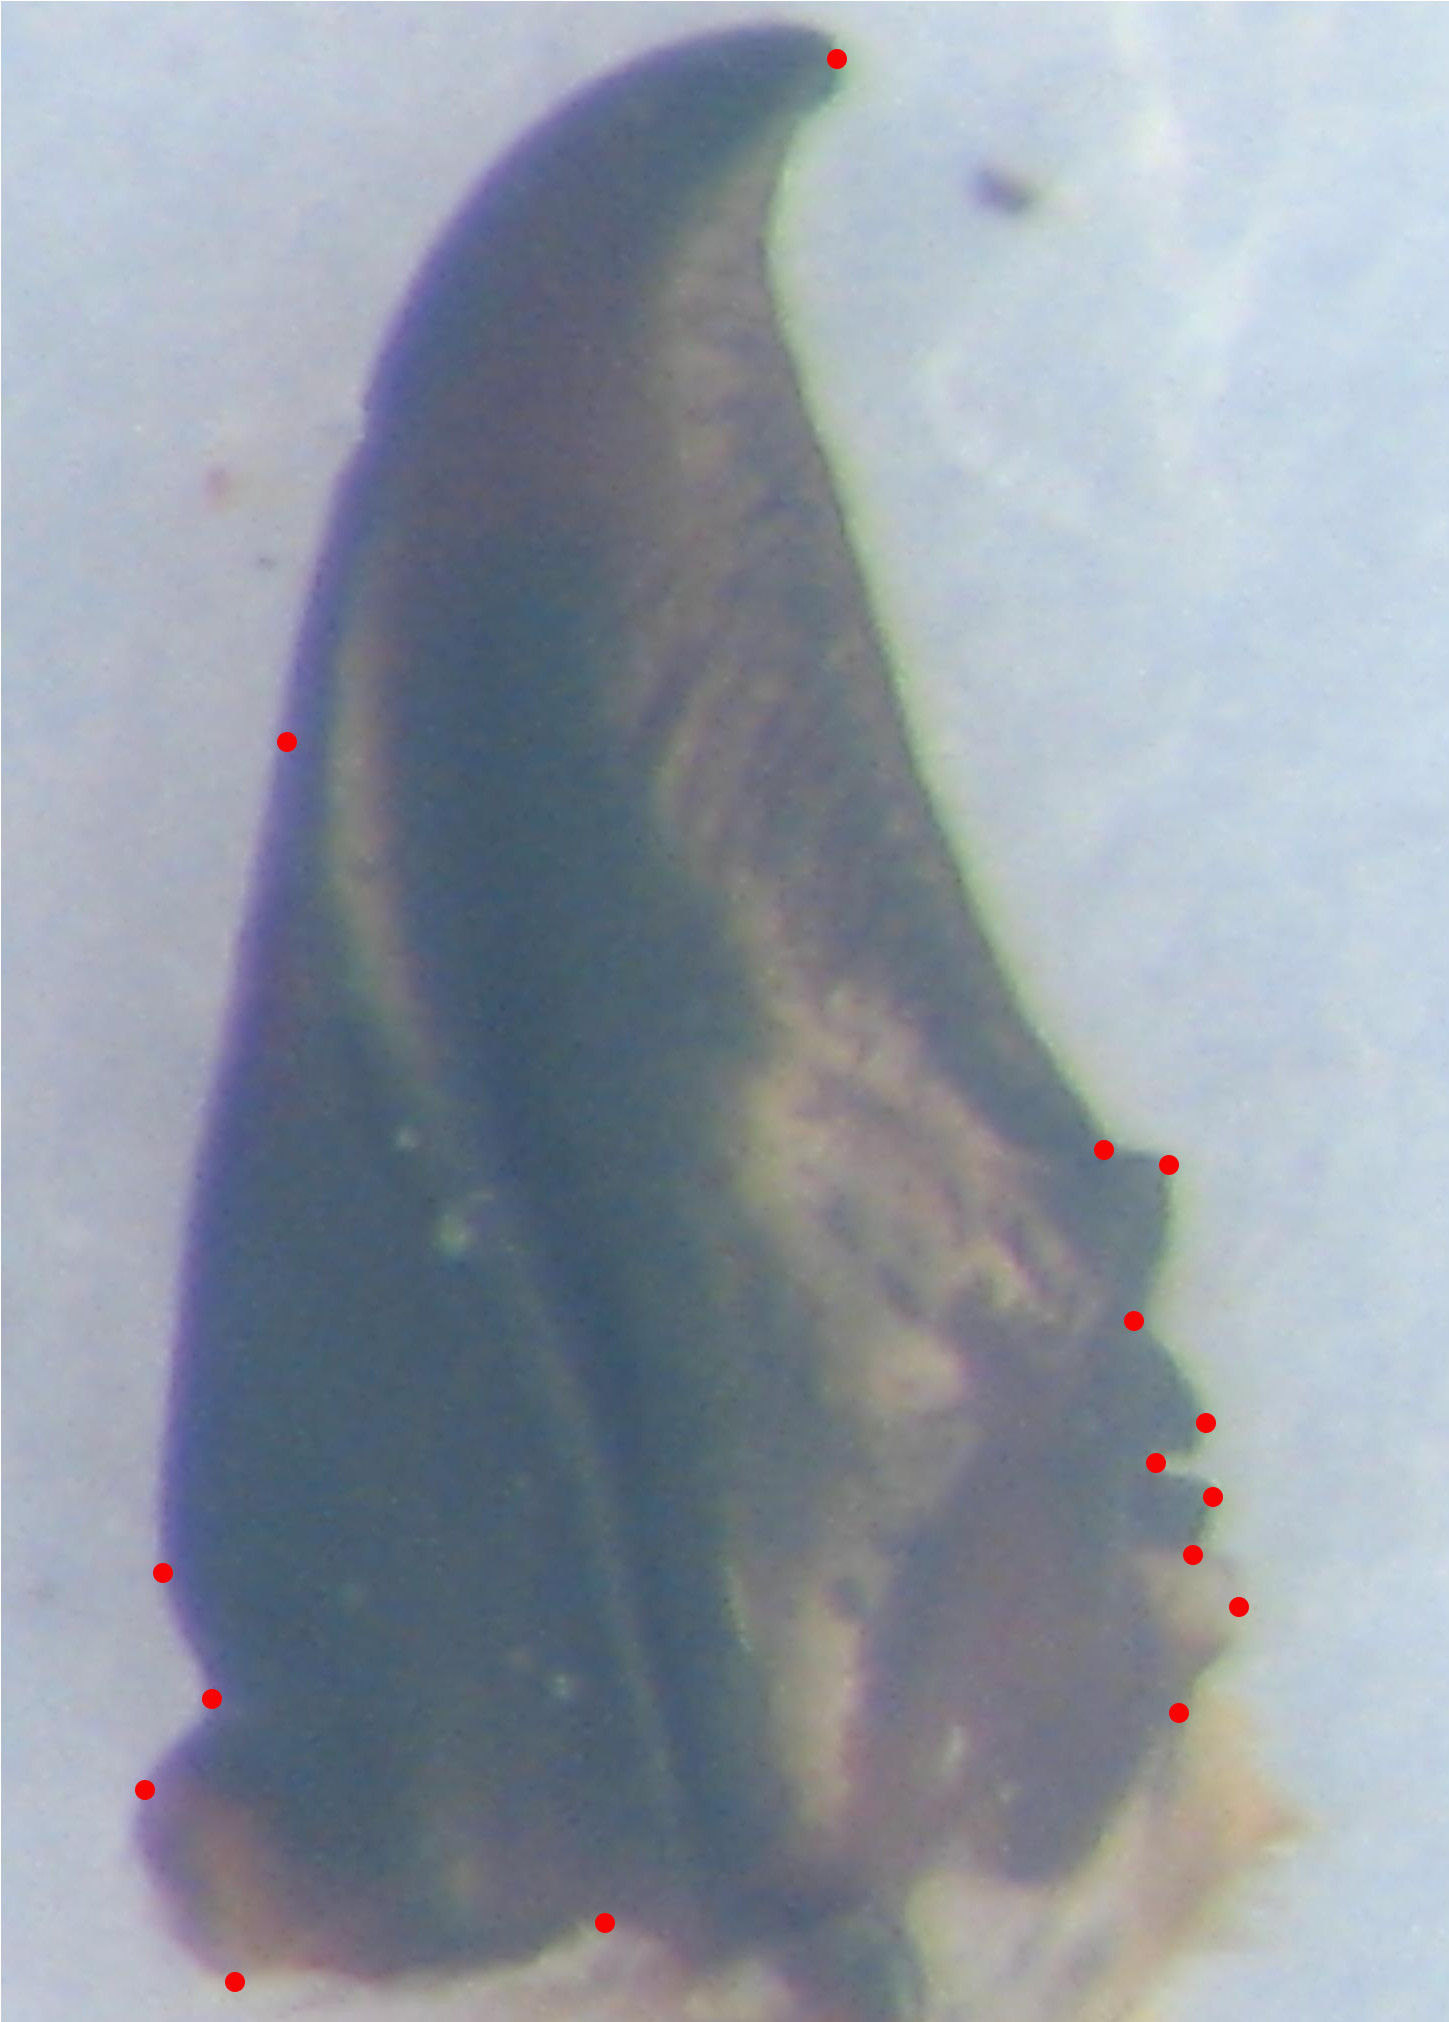
\includegraphics[scale=0.29,valign=m]{./images/mg19_sp}}~~
\subfloat[Right mandible]{\label{figrbox1}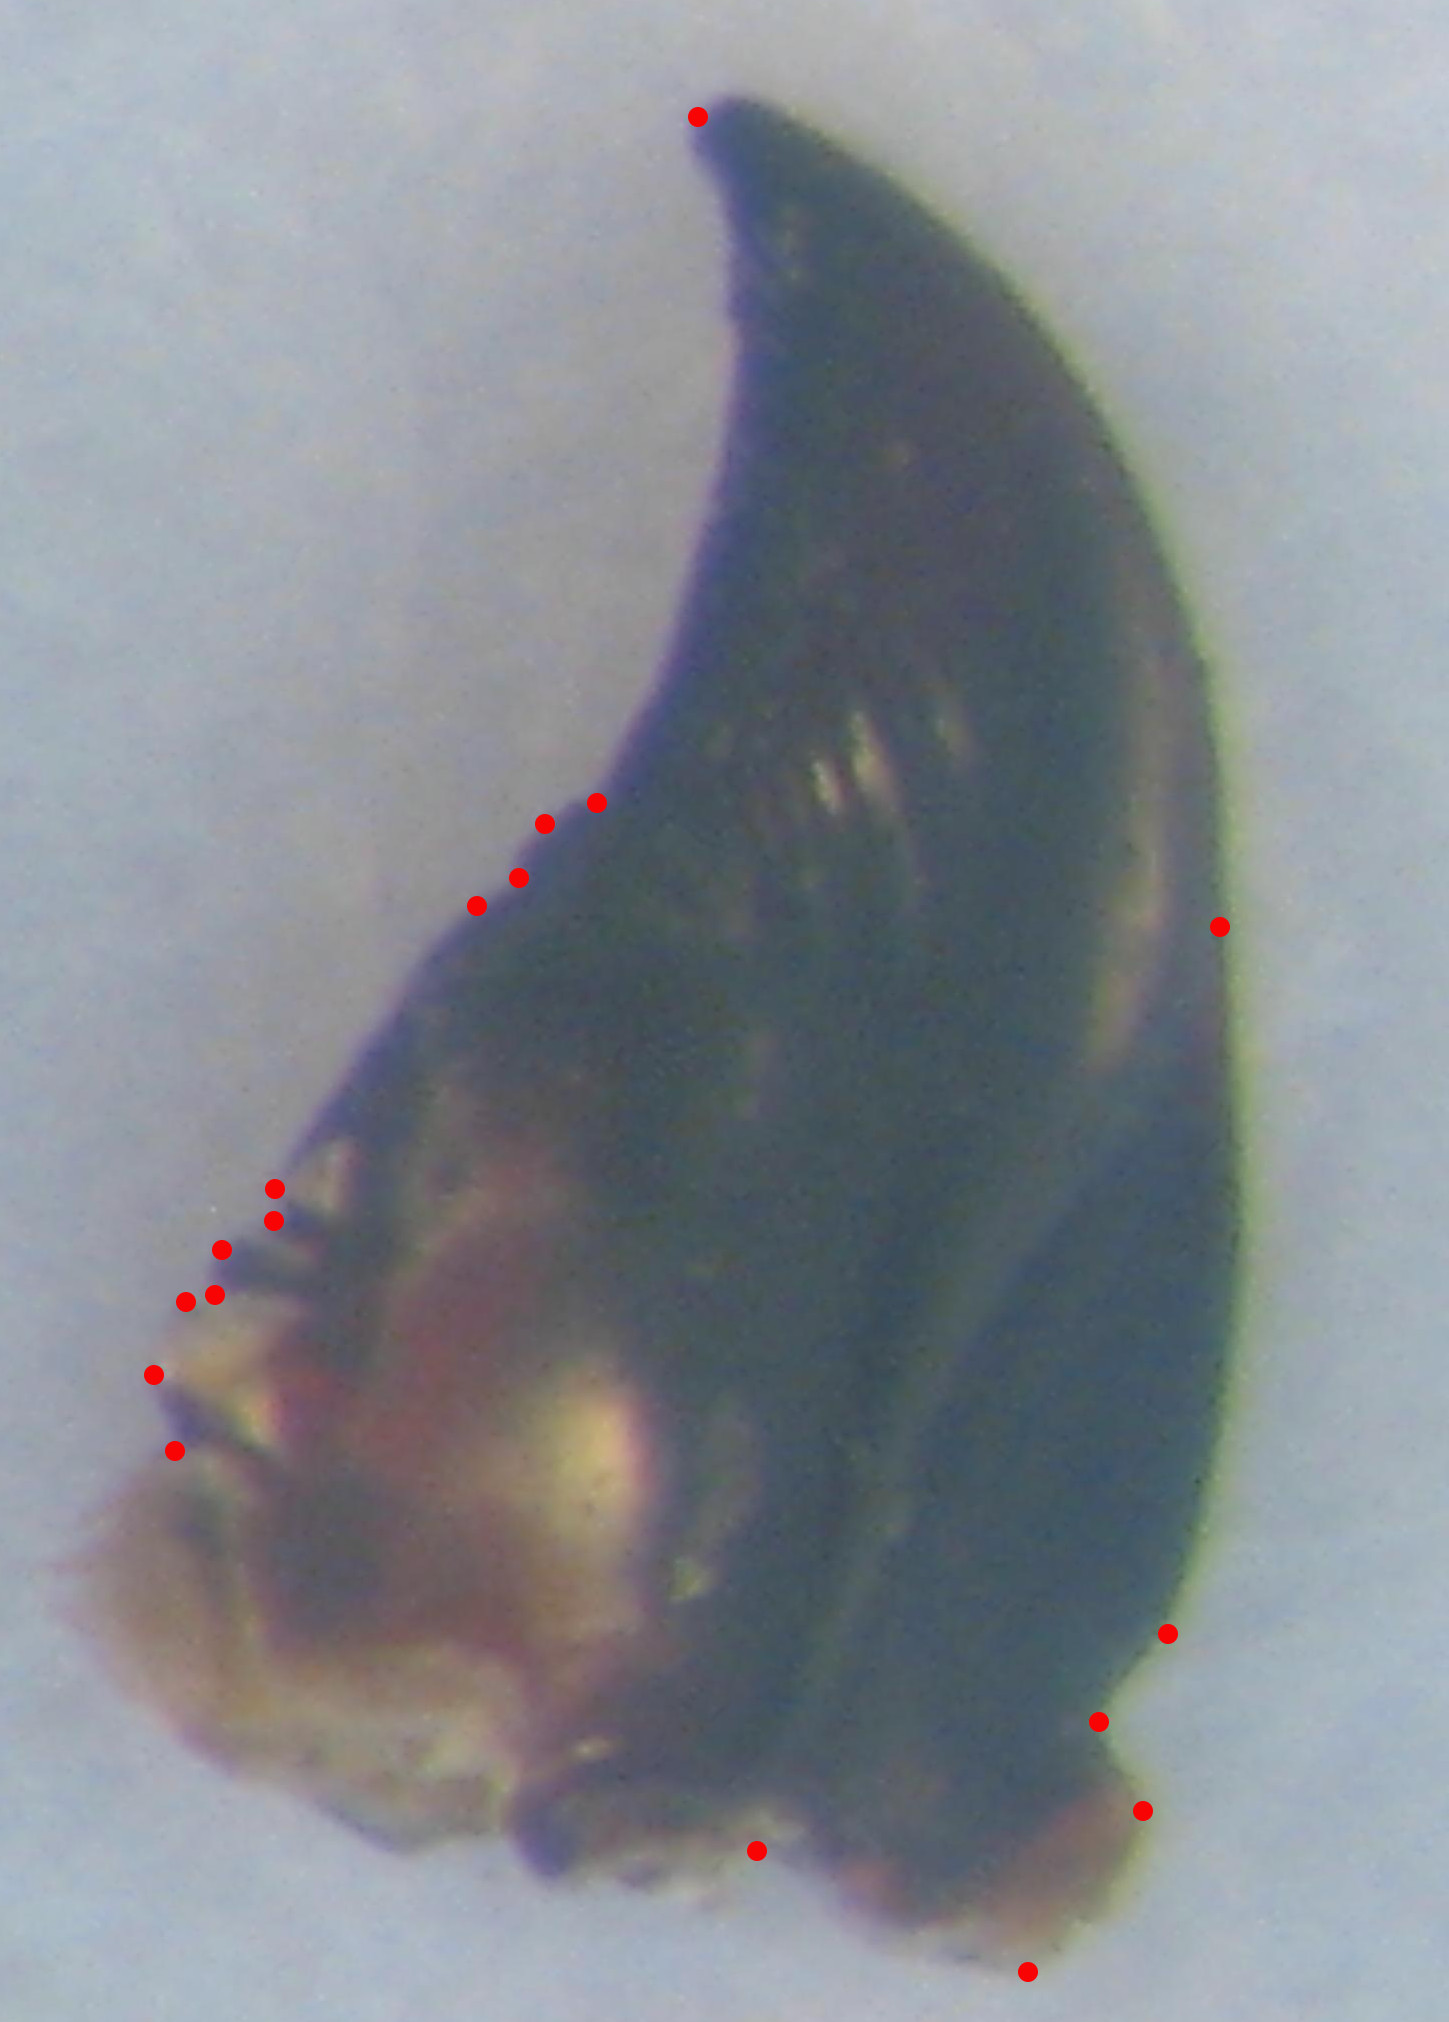
\includegraphics[scale=0.30,valign=m]{./images/md28_sp}}
\caption{Example of beetle mandibles from the studied data set with
  manual landmarks.}
\label{fig1}
\end{figure}
\end{block}
\end{column}
\begin{column}{\sepwidth}\end{column} % Empty spacer column
\begin{column}{\twothirdcolwidth}
\begin{block}{Proposed method}
	\begin{columns}[t]
		\begin{column}{\sepwidth}\end{column}
		\begin{column}{\fourcolwidth}
			\begin{itemize}
				\item \textbf{\underline{Input:}} 
					
					\begin{itemize}\normalsize{
						\item A model image
						\item The manual landmarks of model image
						\item A scene image}
					\end{itemize}
					
					~\\[0.2cm]
				\item \textbf{\underline{Output:}} 
					
					\begin{itemize}\normalsize{
						\item Landmarks of scene image}
					\end{itemize}		  				
					
					~\\[0.3cm]
  				\item \textbf{\underline{Steps:}}
									
  					\begin{itemize}\normalsize{
  						\item Shape identification: segmentation and registration
  						\item SIFT and landmarks: Extract the patches, \\calculate the SIFT descriptors and \\estimate the coordinates of landmarks on the scene image.}
  					\end{itemize}
  					
  					~\\[0.3cm]
			\end{itemize}
		\end{column}
		\begin{column}{\twocolwidth}
		\begin{figure}
				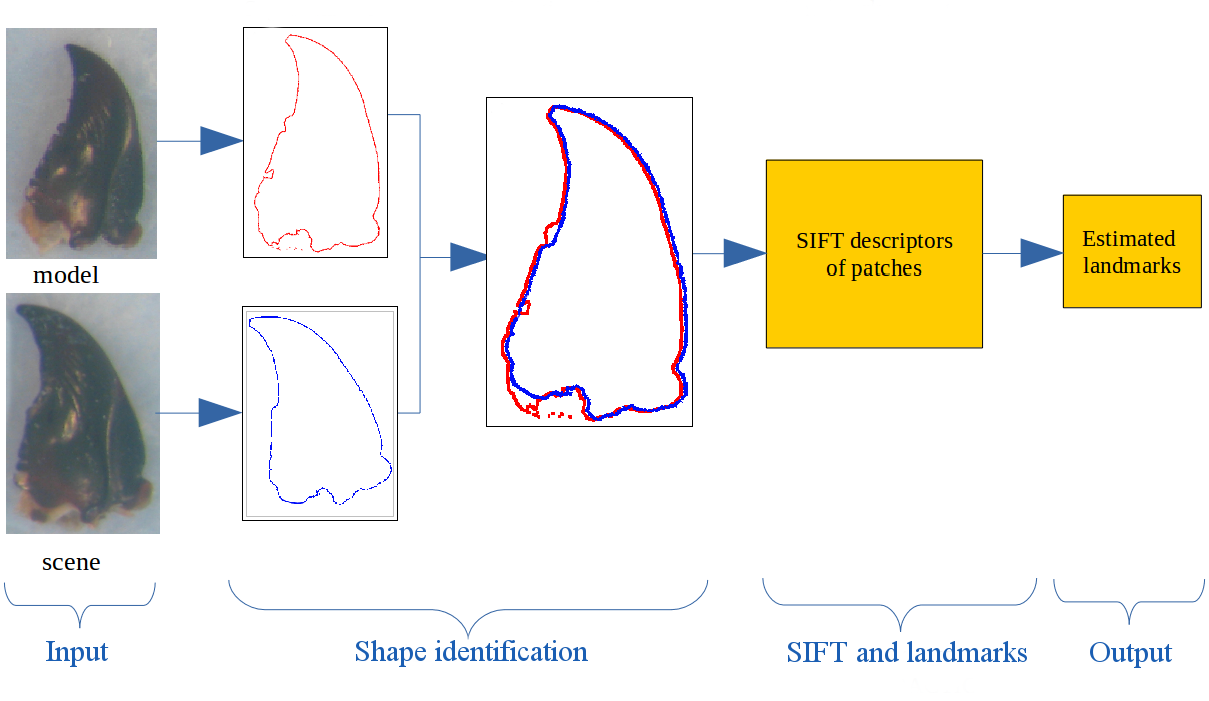
\includegraphics[scale=.70,left,valign=t]{images/method2}
		\end{figure}
		\end{column}
	\end{columns}
	~\\[0.1mm]
\end{block}
\end{column}

%\begin{itemize}
 % 		\item \textbf{\underline{Input:}} 
	%	\begin{itemize}
	%		\item Model image
	%		\item Model manual landmarks
	%		\item Scene image
	%	\end{itemize}		  		
  		
  	%\end{itemize}
	



\begin{column}{\sepwidth}\end{column} % Empty spacer column

\end{columns}

% ------------ Changing number of columns in the width ------------

\begin{columns}[t]

\begin{column}{\sepwidth}\end{column} % Empty spacer column


\begin{column}{\twocolwidth}

\begin{block}{Segmentation}
	
	\begin{enumerate}[\hspace{25pt}1.]
		\item Converting the image to binary one by applying a threshold determined by histogram analysis \cite{beurton2017maelab},
		\item Contours points are extracted by Canny algorithm \cite{canny1986computational}. The thresholds ratio in Canny: $T_{lower} = (1/3) \times T^{upper}$,\\ in which $T^{lower}$ equals to the threshold value in step 1.
	\end{enumerate}
	
\end{block}

%\vspace{5pt}

%\begin{alertblock}{Jean de Nivelle}
%\textbf{Jean de Nivelle} (1422 -- 26 juin 1477) également connu sous le nom de Jean III (Ier) de Montmorency-Nevele, est un personnage français du Moyen Âge (XVe siècle) à l'origine de l'expression populaire \emph{être comme ce chien de Jean de Nivelle (qui fuit quand on l'appelle)} et dont le nom apparaît dans plusieurs chansons traditionnelles françaises.
%\end{alertblock}

\vspace{5pt}

\begin{block}{Registration}
Model and scene images are segmented to extract the contours points. The contours points are registered by applying \textbf{P}rincipal \textbf{C}omponent \textbf{A}nalysis \cite{jolliffe2002principal} \textbf{I}teration (PCAI).
 \begin{enumerate}[\hspace{30pt}1.]
    		\item Compute the centroid point and principal axis of each list of contour points,
    		\item Compute the \textbf{translation} and \textbf{rotation} values between two lists of contour points,
    		\item \textbf{Register} the two lists of contour points,
    		\item Sort the contour points of scene image followed y-direction,
    		\item Select a subset of contour points of scene image and repeat step 1,
    		\item PCAI stop automatically when the \textbf{angle difference} between two 
    	lists of contour points is less than \textbf{$1.5$ degree}.
    \end{enumerate}
\end{block}

\vspace{5pt}

\begin{block}{SIFT and landmarks}
\begin{figure}
    	 \centering
    	 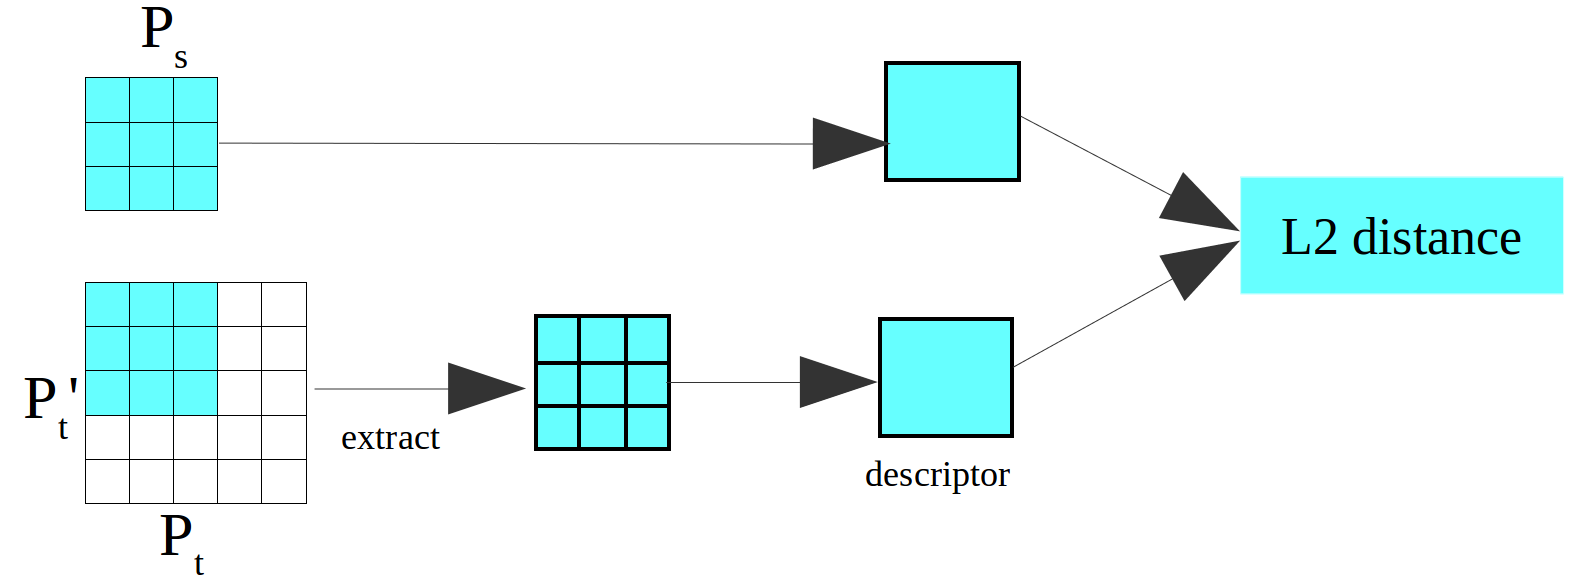
\includegraphics[scale=.7]{images/extract}
    \end{figure}
    \begin{enumerate}[\hspace{25pt}1.]
    		\item A \textbf{patch} $P_s$ is initialized at each manual landmark of model image (size of $9\times9$),
    		\item Calculating the SIFT\cite{lowe1999object} descriptor for $P_s$,
    		\item At the same position in the scene image, a patch $P_t$ is created (size of $36\times36$),
    		\item For each pixel in $P_t$, a patch $P'_t$ is extracted with the same size than $P_s$,
    		\item Calculating the SIFT descriptor for all $P'_t$,
    		\item Computing the distance between the descriptor of $P_s$ and each $P'_t$,
    		\item At the end, the pixel that has the \textbf{minimum distance} with $P_s$ is kept.
    \end{enumerate}
\end{block}

\end{column}

\begin{column}{\sepwidth}\end{column}

\begin{column}{\twocolwidth}

\begin{block}{Results on right mandibles}
	\begin{itemize}
  		\item Highest accuracy: $1^{st}$ landmark with \textbf{$98.62\%$}
  		\item Lowest accuracy: $13^{th}, 14^{th}$ landmark with app. $75\%$
  	\end{itemize}
  	\begin{figure}[l]
		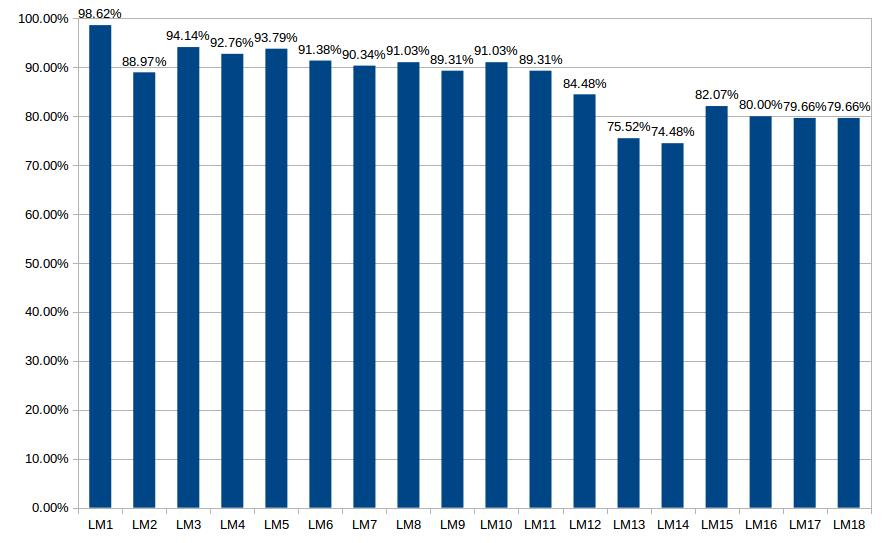
\includegraphics[width=0.6\textwidth]{images/md_chartlms}~~
		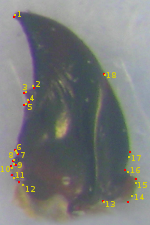
\includegraphics[scale=1.8]{images/md_rs}
	\end{figure}
  	%\Put(740,38){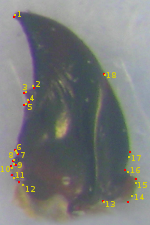
\includegraphics[scale=1.0]{images/md_rs}}
  	%\Put(2,40){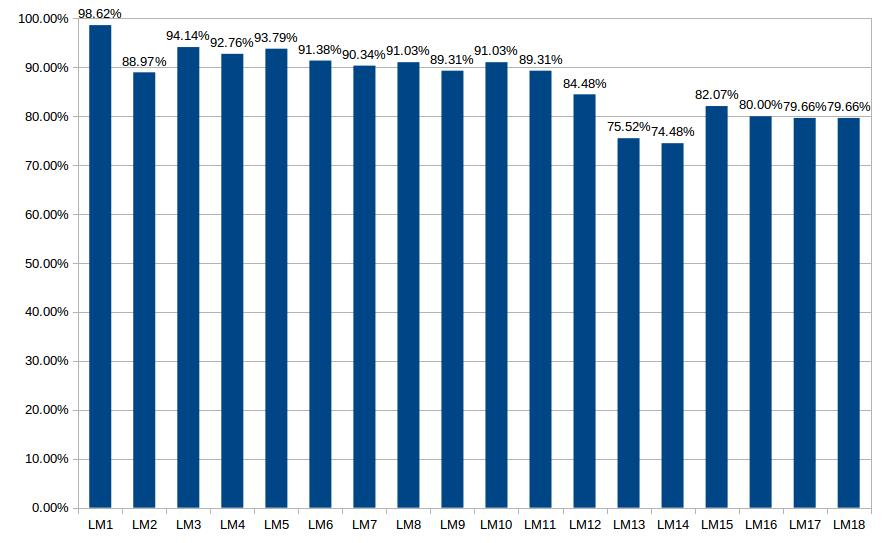
\includegraphics[scale=.6]{images/md_chartlms}}
  	
\end{block}

\begin{block}{Results on left mandibles}
	
	\begin{itemize}
  		\item Highest accuracy: $1^{st}$ landmark with \textbf{$93.01\%$}
  		\item Lowest accuracy: $11^{th}, 12^{th}$ and $16^{th}$ landmark from  $60\%$ to app. $63\%$
  	\end{itemize}
  	\begin{figure}
		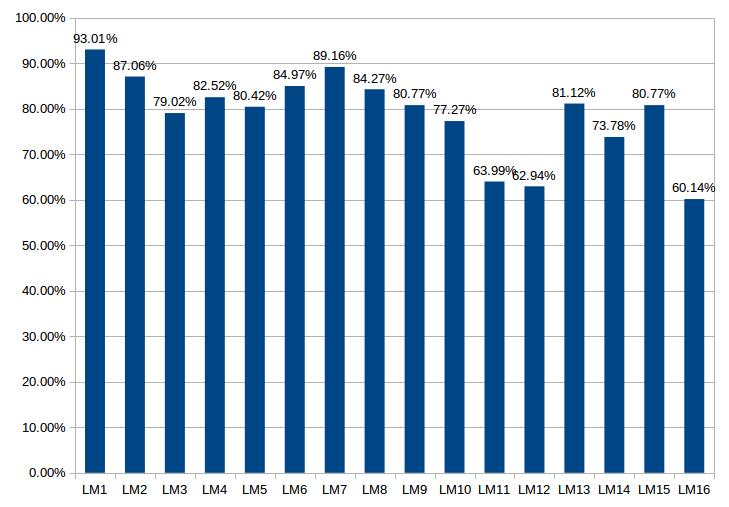
\includegraphics[width=0.61\textwidth]{images/mg_chartlms}~~
		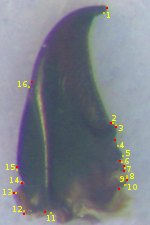
\includegraphics[scale=1.9]{images/mg_rs}
	\end{figure}
\end{block}

\end{column}

\begin{column}{\sepwidth}\end{column}
\end{columns}

% ------------ Changing number of columns in the width ------------


\begin{columns}[t] 

\begin{column}{\sepwidth}\end{column} % Empty spacer column

\begin{column}{\onecolwidth}
\begin{block}{Conclusion}
	\begin{itemize}
		\item A solution based on SIFT descriptor for landmark estimation is presented,
		\item The results show that method \textbf{succeed in locating} all landmarks in  request images,
		\item The accuracy of method is sufficient to be \textbf{proposed to biologists} as a \textbf{replacement of manual positioning}, and to characterize the shape.
	\end{itemize}
\end{block}
\end{column}

\begin{column}{\sepwidth}\end{column} % Empty spacer column

\end{columns}

\begin{columns}[t] 

\begin{column}{\sepwidth}\end{column} % Empty spacer column

\begin{column}{\onecolwidth}
\begin{block}{References}
	\hspace{2cm}
	\begin{multicols}{2}
		\setbeamertemplate{bibliography item}{\insertbiblabel}
		\bibliographystyle{unsrt}
		\bibliography{references}
	\end{multicols}
\end{block}

\end{column}

\begin{column}{\sepwidth}\end{column} % Empty spacer column

\end{columns}


\end{frame}


\end{document}










% ------------ Changing number of columns in the width ------------


\begin{columns}[t]

\begin{column}{\sepwidth}\end{column} % Empty spacer column

\begin{column}{\fourcolwidth}
\begin{block}{L'injonction du Faucon}
L’oiseau chasseur lui dit : 

\begin{quote} Ton peu d’entendement \\
Me rend tout étonné. Vous n’êtes que racaille, \\
Gens grossiers, sans esprit, à qui l’on n’apprend rien. \\
Pour moi, je sais chasser, et revenir au maître. \\
Le vois-tu pas à la fenêtre ? \\
Il t’attend : es-tu sourd ? 
\end{quote}
\end{block}


\begin{block}{La réponse du Chapon}

\begin{quote}
Je n’entends que trop bien,
\end{quote}
Repartit le chapon ; 

\begin{quote}
Mais que me veut-il dire,\\
Et ce beau cuisinier armé d’un grand couteau ?\\
Reviendrais-tu pour cet appeau :
\end{quote}
\end{block}


\end{column}

\begin{column}{\sepwidth}\end{column} % Empty spacer column

\begin{column}{\twocolwidth}

\begin{figure}
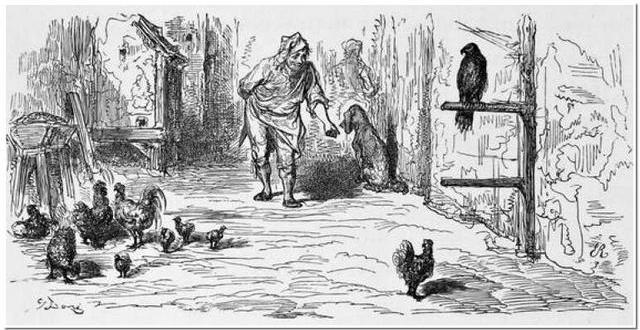
\includegraphics[width=\textwidth]{le-faucon-et-le-chapon-gustave-dore.jpg}
\end{figure}

\begin{block}{L'ironie du Chapon}
\begin{quote}

Laisse-moi fuir ; cesse de rire\\
De l’indocilité qui me fait envoler,\\
Lorsque d’un ton si doux on s’en vient m’appeler.
\end{quote}
\end{block}

\end{column}

\begin{column}{\sepwidth}\end{column} % Empty spacer column

\begin{column}{\fourcolwidth}

\begin{block}{La conclusion du Chapon}

\begin{quote}
Si tu voyais mettre à la broche \\
Tous les jours autant de faucons \\
Que j’y vois mettre de chapons, \\
Tu ne me ferais pas un semblable reproche. 
\end{quote}
\end{block}


\begin{block}{Oiseau Tikz}
\begin{figure}[ht!]
\begin{center}
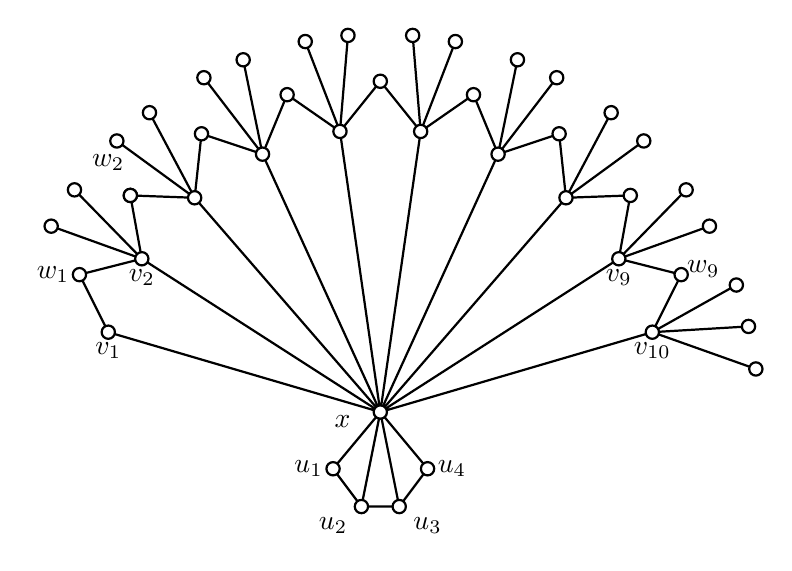
\begin{tikzpicture}[scale=1.2,style=thick]
\def\vr{2pt} % \vr = vertex radius;  Set \vr = 2/scale for uniform sizing
of vertices
%%% define points
\path (0,0) coordinate (x);
%%%


\path (x) +(-180-180/11:3) coordinate (v1);
\path (x) +(-180-180*2/11:3) coordinate (v2);
\path (x) +(-180-180*3/11:3) coordinate (v3);
\path (x) +(-180-180*4/11:3) coordinate (v4);
\path (x) +(-180-180*5/11:3) coordinate (v5);
\path (x) +(-180-180*6/11:3) coordinate (v6);
\path (x) +(-180-180*7/11:3) coordinate (v7);
\path (x) +(-180-180*8/11:3) coordinate (v8);
\path (x) +(-180-180*9/11:3) coordinate (v9);
\path (x) +(-180-180*10/11:3) coordinate (v10);
%%%
\path (x) +(-180-180*1.5/11:3.5) coordinate (w1);
\path (x) +(-180-180*2.5/11:3.5) coordinate (w2);
\path (x) +(-180-180*3.5/11:3.5) coordinate (w3);
\path (x) +(-180-180*4.5/11:3.5) coordinate (w4);
\path (x) +(-180-180*5.5/11:3.5) coordinate (w5);
\path (x) +(-180-180*6.5/11:3.5) coordinate (w6);
\path (x) +(-180-180*7.5/11:3.5) coordinate (w7);
\path (x) +(-180-180*8.5/11:3.5) coordinate (w8);
\path (x) +(-180-180*9.5/11:3.5) coordinate (w9);
%%%
\path (x) +(-180-180*1.8/11:4) coordinate (a2);
\path (x) +(-180-180*2.2/11:4) coordinate (b2);
\path (x) +(-180-180*2.8/11:4) coordinate (a3);
\path (x) +(-180-180*3.2/11:4) coordinate (b3);
\path (x) +(-180-180*3.8/11:4) coordinate (a4);
\path (x) +(-180-180*4.2/11:4) coordinate (b4);
\path (x) +(-180-180*4.8/11:4) coordinate (a5);
\path (x) +(-180-180*5.2/11:4) coordinate (b5);
\path (x) +(-180-180*5.8/11:4) coordinate (a6);
\path (x) +(-180-180*6.2/11:4) coordinate (b6);
\path (x) +(-180-180*6.8/11:4) coordinate (a7);
\path (x) +(-180-180*7.2/11:4) coordinate (b7);
\path (x) +(-180-180*7.8/11:4) coordinate (a8);
\path (x) +(-180-180*8.2/11:4) coordinate (b8);
\path (x) +(-180-180*8.8/11:4) coordinate (a9);
\path (x) +(-180-180*9.2/11:4) coordinate (b9);
\path (x) +(-180-180*9.8/11:4) coordinate (a10);
\path (x) +(-180-180*10.2/11:4) coordinate (b10);
\path (x) +(-180-180*10.6/11:4) coordinate (c10);
%%% body of the peacock
\path (-0.5,-0.6) coordinate (leg1);
\path (-0.2,-1) coordinate (leg2);
\path (0.2,-1) coordinate (leg3);
\path (0.5,-0.6) coordinate (leg4);
%%% Edges:
\draw (v1) -- (x) -- (v2);
\draw (v3) -- (x) -- (v4);
\draw (v5) -- (x) -- (v6);
\draw (v7) -- (x) -- (v8);
\draw (v9) -- (x) -- (v10);
%%%
\draw (v1) -- (w1) -- (v2) -- (w2) -- (v3) -- (w3) -- (v4) -- (w4) -- (v5) -- (w5) -- (v6) -- (w6) -- (v7) -- (w7) -- (v8) -- (w8) -- (v9) -- (w9) -- (v10);
%%%
\draw (a2) -- (v2) -- (b2);
\draw (a3) -- (v3) -- (b3);
\draw (a4) -- (v4) -- (b4);
\draw (a5) -- (v5) -- (b5);
\draw (a6) -- (v6) -- (b6);
\draw (a7) -- (v7) -- (b7);
\draw (a8) -- (v8) -- (b8);
\draw (a9) -- (v9) -- (b9);
\draw (a10) -- (v10) -- (b10);
\draw (v10) -- (c10);
%%%
\draw (leg1) -- (leg2) -- (leg3) -- (leg4);
\draw (leg1) -- (x) -- (leg2);
\draw (leg3) -- (x) -- (leg4);
%%% Vertices:
\draw (x) [fill=white] circle (\vr);
\draw (v1) [fill=white] circle (\vr); \draw (v2) [fill=white] circle (\vr);
\draw (v3) [fill=white] circle (\vr); \draw (v4) [fill=white] circle (\vr);
\draw (v5) [fill=white] circle (\vr); \draw (v6) [fill=white] circle (\vr);
\draw (v7) [fill=white] circle (\vr); \draw (v8) [fill=white] circle (\vr);
\draw (v9) [fill=white] circle (\vr); \draw (v10) [fill=white] circle (\vr);
%%%
\draw (w1) [fill=white] circle (\vr); \draw (w2) [fill=white] circle (\vr);
\draw (w2) [fill=white] circle (\vr); \draw (w3) [fill=white] circle (\vr);
\draw (w4) [fill=white] circle (\vr); \draw (w5) [fill=white] circle (\vr);
\draw (w6) [fill=white] circle (\vr); \draw (w7) [fill=white] circle (\vr);
\draw (w8) [fill=white] circle (\vr); \draw (w9) [fill=white] circle (\vr);
%%%
\draw (a2) [fill=white] circle (\vr); \draw (b2) [fill=white] circle (\vr);
\draw (a3) [fill=white] circle (\vr); \draw (b3) [fill=white] circle (\vr);
\draw (a4) [fill=white] circle (\vr); \draw (b4) [fill=white] circle (\vr);
\draw (a5) [fill=white] circle (\vr); \draw (b5) [fill=white] circle (\vr);
\draw (a6) [fill=white] circle (\vr); \draw (b6) [fill=white] circle (\vr);
\draw (a7) [fill=white] circle (\vr); \draw (b7) [fill=white] circle (\vr);
\draw (a8) [fill=white] circle (\vr); \draw (b8) [fill=white] circle (\vr);
\draw (a9) [fill=white] circle (\vr); \draw (b9) [fill=white] circle (\vr);
\draw (a10) [fill=white] circle (\vr); \draw (b10) [fill=white] circle (\vr);
\draw (c10) [fill=white] circle (\vr);
%%% 
\draw (leg1) [fill=white] circle (\vr);
\draw (leg2) [fill=white] circle (\vr);
\draw (leg3) [fill=white] circle (\vr);
\draw (leg4) [fill=white] circle (\vr);
%%% text
\draw (-0.4,-0.1) node {$x$};
\draw [below] (v1) node {$v_1$};
\draw [below] (v2) node {$v_2$};
\draw [below] (v9) node {$v_9$};
\draw [below] (v10) node {$v_{10}$};
\draw [left] (w1) node {$w_1$};
\draw (w2) node[xshift=-8pt, yshift=12pt] {$w_2$};
\draw (w9) node[xshift=8pt, yshift=2pt] {$w_9$};
\draw [left] (leg1) node {$u_1$};
\draw (-0.5,-1.2) node {$u_2$};
\draw (0.5,-1.2) node {$u_3$};
\draw [right] (leg4) node {$u_4$};
\end{tikzpicture}
\end{center}
\end{figure}
Certes cet oiseau ne ressemble ni à un chapon, ni à un faucon. Léon! Serait-ce un Paon?
\end{block}

\end{column}


\begin{column}{\sepwidth}\end{column} % Empty spacer column

\end{columns}